

\section{Theorie}
\label{sec:Theorie}
Mit Drehmoment $\vec{M}$ Trägheitsmoment $I$ und Winkelbeschleunigung $\dot{\omega}$
lassen sich Dynamische Rotationsbewegungen beschreiben. Das Trägheitsmoment ist
durch
\begin{equation}
  I=\sum_i r_1^2m_i=\int r^2 \text{d}m
\end{equation}
gegeben.
Beispiele für trägheitsmomente sind
\begin{figure}
  \centering
  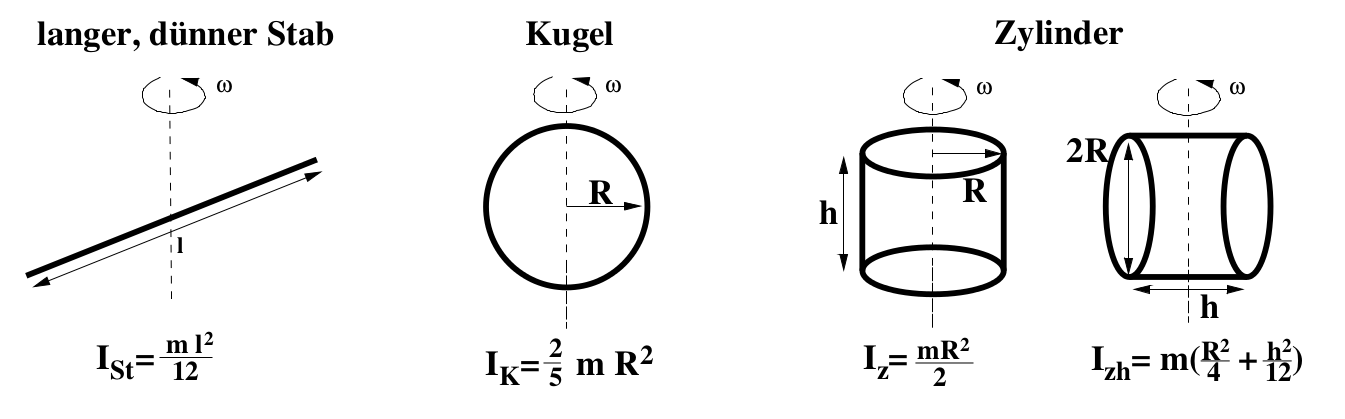
\includegraphics[width=0.9\textwidth]{Traegheitsmomente.png}
  \caption{Trägheitsmomente für verschiedene Körper \cite{sample}.}
  \label{fig:Traegheitsmomente}
\end{figure}
Ist ein Körper dessen Trägheitsmoment bekannt ist, von der Drehachse um
$a$ verschoben so lasst sich das neue Trägheitsmoment berechnen durch den
Steinerschen satz
\begin{equation}
  I=I_s+m a^2
\end{equation}
Das Drehmoment M berechnet sich durch
\begin{equation}
  \vec{M}=\vec{F}\times\vec{r}
\end{equation}
Wenn in einem System eine zum Auslenkungswinkel $\phi$ Rücktreibende Kraft
existiert, führt das System eine Schwingung mit der Schwingungsdauer
\begin{equation}
  T=2\pi\sqrt{\frac{I}{D}}
  \label{eqn:Periodetorrosion}
\end{equation}
Diese Gleichung ist eine näherung für kleine Winkel
Das durch die Rücktreibende Kraft erzeugte Drehmoment ist bestimmt durch
\begin{equation}
  M=D \phi
  \label{eqn:Traegheitmomenttorrosion}
\end{equation}
Mit den Gleichungen \eqref{eqn:Traegheitmomenttorrosion} \eqref{eqn:Periodetorrosion}
lassen sich auch die Winkelrichtgrößen $D$ von Torrosionsfedern
berechnen.
\begin{equation}
  D=\frac{Fr}{\phi}
  \label{eqn:Winkelrichtgroesse}
\end{equation}
  \cite{sample}
